\documentclass[
	12pt,
	oneside,
	bibliography=totocnumbered]{scrartcl}


\usepackage{amsmath}


% formatting the captions of figures
\usepackage[bf]{caption} % make headings boldfont

% for drawing :-)
\usepackage{tikz} 
\usetikzlibrary{backgrounds} % to have a background layer
\usepackage{xcolor} % defining my own colors
\usetikzlibrary{positioning} % arrows between nodes and relative positions



% for drawing from different lotteries (left/right)
\usepackage{xifthen}

% Define colors
\colorlet{sampleShade}{gray!40}  % shading of sample trials
\colorlet{choiceShade}{blue!40}  % shading of choice trials
\colorlet{choiceCol}{red!70} % color of chosen option



% Some variables for drawing
\newcommand\sideAdj{13}


% For figures
\usepackage{graphicx}
\graphicspath{{./figures/}} % specify relative path with extra {}


% For references
\usepackage[
	backend=biber, % troubleshooting: http://tex.stackexchange.com/questions/154751/biblatex-with-biber-configuring-my-editor-to-avoid-undefined-citations
	style=numeric-comp]{biblatex}

\addbibresource{DFE_refs.bib}


% For hyperlinks in table of contents, and references
\usepackage{hyperref}
\hypersetup{
    colorlinks,
    citecolor=black,
    filecolor=black,
    linkcolor=black,
    urlcolor=black}


% General document info
\title{Terminating Information Search}
\author{Stefan Appelhoff}



%%%%%%%%%%%%%%%%%%%%%%%%%%%%%%%%%%%%%%%%%%%%%%%%%%%%%%%%%%%%%%


\begin{document}
\maketitle
\tableofcontents



\section{Introduction}

As agents in different environments, humans often find themselves in situations that require decisions based on limited knowledge about the available choice options. The topic of the present project is the process, how humans selectively sample choice options to arrive at a more refined knowledge about the properties of the options. Specifically, the interest lies in self-directed information search in sequential decision making problems. A short example illustrates the topic further: 

\begin{quotation}
Imagine that your laptop is broken and you want to acquire a new one. In the process, you may sequentially sample several available models and their respective properties such as prices, specifications, and reviews. To avoid indefinite browsing, you will need to terminate your search at some point and select a new laptop - most likely without having obtained full certainty about the best option.
\end{quotation} 

For the project described here, the aforementioned example will be transformed into an experimental paradigm that allows for the examination of behavioral and neural aspects of choice in a controled manner. Similar to the real life example, the experimental paradigm exhibits the following characteristics:

\begin{itemize}
\item There is an environment in which several options exist that will yield outcomes upon selection.
\item There exists limited knowledge about the options and the frequencies of their associated outcomes.
\item There will be the opportunity to obtain information about the options through a sampling of the options.
\item The overall goal is to maximize the positive outcomes obtained from the options in the long run.
\end{itemize}

In the paradigm, participants will make sequential decisions about which option to sample. In these trial to trial decisions, the question of interest to this project lies in how participants set their termination criteria. I.e., when do participants decide to terminate the information search in one option and switch to search another option? When do participants decide to stop sampling altogether and decide for one final option to be optimal based on current knowledge? The remainder of this document will be a concise formulation of the research questions followed by an outline of the experimental paradigm. Finally, the implementation of the experimental paradigm on a computer program will be described.


\section{Research Questions}

% Listing the research questions
\begin{enumerate}
\item How are sampling efforts sequentially allocated to the different options?
\item How do we arrive at a decision to terminate the information search?
\item What is the quantitative link between neural signals obtained by EEG with the behavioral data of participants performing the experimental paradigm.
\end{enumerate}



\section{The Experimental Paradigm}
The proposed experiment will be based on a combination  of two different paradigms that are well known in the literature.

\begin{enumerate}
\item The n-armed Bandit Paradigm
\item The Sampling Paradigm
\end{enumerate}

In the following, these two paradigms will be descibed in detail. Figure \ref{fig:paradigms} provides an overview of the paradigms.


% Start the paradigm figure
% -------------------------------------------------
% -------------------------------------------------
% we want random values
\pgfmathsetseed{9999}
\pgfmathdeclarerandomlist{badLottery}{{0}{0}{0}{0}{0}{0}{0}{1}{1}{1}}
\pgfmathdeclarerandomlist{goodLottery}{{1}{1}{1}{1}{1}{1}{1}{0}{0}{0}}


\begin{figure}[t]
\begin{center}
\resizebox{.9\linewidth}{!}{%
\begin{tikzpicture}

% --------------------------------------------------%
%		 Begin with a general case   			   %
% --------------------------------------------------%


% TO DO

% figure part indication
\node [scale=1.5]at (0,20) {\textbf{A)}};

% drawing two initial rectangles as environment
\filldraw [color=black, fill=white](4,15) rectangle (5,16)node[above, scale=1.5]{\textbf{Environment}};
\filldraw [color=black, fill=white](5,15) rectangle (6,16);


% now "left choice" rectangles
\filldraw [color=black, fill=choiceCol](10,17) rectangle (11,18)node[above, scale=1.5]{\textbf{Choose Left}};
\filldraw [color=black, fill=white](11,17) rectangle (12,18);


% now "right choice" rectangles
\filldraw [color=black, fill=white](10,13) rectangle (11,14) node[above, scale=1.5]{\textbf{Choose Right}};
\filldraw [color=black, fill=choiceCol](11,13) rectangle (12,14);



\begin{scope}[on background layer]
% Drawing lines to the choice rectangles
\draw [line width=0.5mm](6,15.5) -- (10.01,17.5);
\draw [line width=0.5mm](6,15.5) -- (10.01,13.5);

% Drawing lines to outcome probabilities 
\draw [line width=0.5mm](12,13.5) -- (16,14.5) node[right, scale=1.5]{$\Pr({1 \mid right})=0.3$};
\draw [line width=0.5mm](12,13.5) -- (16,12.5)node[right, scale=1.5]{$\Pr({0 \mid right})=0.7$};

\draw [line width=0.5mm](12,17.5) -- (16,18.5)node[right, scale=1.5]{$\Pr({1 \mid left})=0.7$};
\draw [line width=0.5mm](12,17.5) -- (16,16.5)node[right, scale=1.5]{$\Pr({0 \mid left})=0.3$};

\end{scope}

% --------------------------------------------------%
%		 Continue with the Bandit Paradigm 		   %
% --------------------------------------------------%



% figure part indication
\node [scale=1.5]at (0,10) {\textbf{B)}};

% figure label
\node [scale=1.5, fill=choiceShade, right] at (8,8) {\textbf{Choice}};

% "direction of time"
\draw [line width=0.5mm,->] (8,8.8) -- (4,0) node [below,scale=1.5] {\textbf{Time}};

% the variables for all rectangles	
\foreach \x/\y/\filColLeft/\filColRight/\labelColLeft/\labelColRight/\action in {
4/8.8/choiceCol/white/black/white/left,
3.5/7.7/choiceCol/white/black/white/left, 
3/6.6/choiceCol/white/black/white/left, 
2.5/5.5/choiceCol/white/black/white/left, 
2/4.4/choiceCol/white/black/white/left, 
1.5/3.3/white/choiceCol/white/black/right, 
1/2.2/choiceCol/white/black/white/right, 
0.5/1.1/white/choiceCol/white/black/right, 
0/0/white/choiceCol/white/black/right}
{

% Draw a random number based on action
\ifthenelse{\equal{\action}{left}}{\pgfmathrandomitem{\outcome}{goodLottery}}{\pgfmathrandomitem{\outcome}{badLottery}};

% background shading
\begin{scope}[on background layer]
\fill [fill=choiceShade](\x-0.15,\y-0.15) rectangle (\x+2.15,\y+1.15);
\end{scope}

% all rectangles in a loop
\filldraw [color=black, fill=\filColLeft](\x,\y) rectangle (\x+1,\y+1) node[midway, color=\labelColLeft] {\textbf{\outcome}};

\filldraw [color=black, fill=\filColRight](\x+1,\y+1) rectangle (\x+2,\y) node[midway, color=\labelColRight] {\textbf{\outcome}};

}



%--------------------------------------------------%
%	      Now the Sampling Paradigm 			      %
%--------------------------------------------------%


% figure part indication
\node [scale=1.5]at (0+\sideAdj,10) {\textbf{C)}};

% figure labels
\node [scale=1.5, fill=sampleShade,right]at (8+\sideAdj,8) {\textbf{Sampling}};

\node [scale=1.5, fill=choiceShade,right]at (5+\sideAdj,1) {\textbf{Choice}};

% direction of time
\draw [line width=0.5mm,->] (8+\sideAdj,8.8) -- (4+\sideAdj,0) node [below,scale=1.5] {\textbf{Time}};

	
% the variables for all rectangles	
\foreach \x/\y/\filColLeft/\filColRight/\labelColLeft/\labelColRight/\action in { 
4+\sideAdj/8.8/choiceCol/white/black/white/left,
3.5+\sideAdj/7.7/white/choiceCol/white/black/right,
3+\sideAdj/6.6/white/choiceCol/white/black/right,
2.5+\sideAdj/5.5/white/choiceCol/white/black/right,
2+\sideAdj/4.4/choiceCol/white/black/white/left,
1.5+\sideAdj/3.3/white/choiceCol/white/black/left,
1+\sideAdj/2.2/choiceCol/white/black/white/left}
{

% Draw a random number based on action
\ifthenelse{\equal{\action}{left}}{\pgfmathrandomitem{\outcome}{goodLottery}}{\pgfmathrandomitem{\outcome}{badLottery}};


% background shading
\begin{scope}[on background layer]
\fill [fill=sampleShade](\x-0.15,\y-0.15) rectangle (\x+2.15,\y+1.15);
\end{scope}

% drawing all the rectangles
\filldraw [color=black, fill=\filColLeft](\x,\y) rectangle (\x+1,\y+1) node[midway, color=\labelColLeft] {\textbf{\outcome}};

\filldraw [color=black, fill=\filColRight](\x+1,\y+1) rectangle (\x+2,\y) node[midway, color=\labelColRight] {\textbf{\outcome}};

}


% drawing the choice rectangles
\filldraw [color=black, fill=choiceCol](0+\sideAdj,0) rectangle (\sideAdj+1,1) node[midway, color=black] {\textbf{1}};

\filldraw [color=black, fill=white](\sideAdj+1,1) rectangle (\sideAdj+2,0) node[midway, color=white] {\textbf{1}};

% background shading of choice rectangle
\begin{scope}[on background layer]
\fill [fill=choiceShade](\sideAdj-0.15,-0.15) rectangle (\sideAdj+2.15,1.15);
\end{scope}

%--------------------------------------------------%
\end{tikzpicture}
} % closing bracket from scaling

\captionsetup{width=.9\linewidth, format=plain}
\caption[Experimental Paradigms]{\textbf{A)} Depiction of a two-armed Bandit. Note that the number of options in the environment can be extended arbitrarily to form an n-armed Bandit. Each Option contains its own probability mass function (pmf) of outcomes. These pmfs are unknown to a subject performing the Bandit task. \textbf{B)} A typical run of trials in a Bandit task. A subject sequentially chooses among options and is provided with feedback. Each trial represents a exploration-exploitation problem.  \textbf{C)} A typical run of trials in the Sampling Paradigm. A subject is allowed to sample the available options without an impact of the outcomes on the final payoff. At some point, the subject can decide to terminate sampling and choose one of the options, which will impact the final payoff.}
\label{fig:paradigms}
\end{center}
\end{figure}


\subsection{The n-armed Bandit Paradigm}
From Hertwig also known as Partial-Feedback-Paradigm \cite{hertwig2009}.






\subsection{The Sampling Paradigm}
yep, pretty nice.





\subsection{Combination of the Two Paradigms}

Need a figure here for the 2x2 design

\begin{figure}[h]
\begin{center}
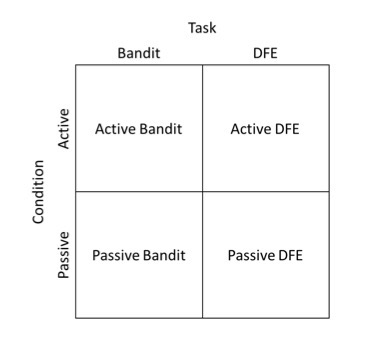
\includegraphics[scale=.5]{2x2_dummy}
\end{center}
\end{figure}





\section{Computerized Implementation of the Experiment}
describe the computer code here

need a figure for the flow ???


\printbibliography

\end{document}